% !TEX encoding = UTF-8 Unicode
\documentclass[a4paper]{article}

\usepackage{color}
\usepackage{url}
\usepackage[T2A]{fontenc} % enable Cyrillic fonts
\usepackage[utf8]{inputenc} % make weird characters work
\usepackage{graphicx}
\usepackage{subcaption}
\usepackage{amsthm}
\usepackage{booktabs}
\usepackage{algorithm}
\usepackage{algpseudocode}


\usepackage[english,serbian]{babel}
%\usepackage[english,serbianc]{babel} %ukljuciti babel sa ovim opcijama, umesto gornjim, ukoliko se koristi cirilica

\usepackage[unicode]{hyperref}
\hypersetup{colorlinks,citecolor=green,filecolor=green,linkcolor=blue,urlcolor=blue}

\usepackage{listings}

%\newtheorem{primer}{Пример}[section] %ćirilični primer
\newtheorem{lemma}{Lema}
\newtheorem{corollary}{Posledica}[lemma]  % corollary numbering is tied to lemma


\definecolor{mygreen}{rgb}{0,0.6,0}
\definecolor{mygray}{rgb}{0.5,0.5,0.5}
\definecolor{mymauve}{rgb}{0.58,0,0.82}

\lstset{ 
  backgroundcolor=\color{white},   % choose the background color; you must add \usepackage{color} or \usepackage{xcolor}; should come as last argument
  basicstyle=\scriptsize\ttfamily,        % the size of the fonts that are used for the code
  breakatwhitespace=false,         % sets if automatic breaks should only happen at whitespace
  breaklines=true,                 % sets automatic line breaking
  captionpos=b,                    % sets the caption-position to bottom
  commentstyle=\color{mygreen},    % comment style
  deletekeywords={...},            % if you want to delete keywords from the given language
  escapeinside={\%*}{*)},          % if you want to add LaTeX within your code
  extendedchars=true,              % lets you use non-ASCII characters; for 8-bits encodings only, does not work with UTF-8
  firstnumber=1000,                % start line enumeration with line 1000
  frame=single,	                   % adds a frame around the code
  keepspaces=true,                 % keeps spaces in text, useful for keeping indentation of code (possibly needs columns=flexible)
  keywordstyle=\color{blue},       % keyword style
  language=Python,                 % the language of the code
  morekeywords={*,...},            % if you want to add more keywords to the set
  numbers=left,                    % where to put the line-numbers; possible values are (none, left, right)
  numbersep=5pt,                   % how far the line-numbers are from the code
  numberstyle=\tiny\color{mygray}, % the style that is used for the line-numbers
  rulecolor=\color{black},         % if not set, the frame-color may be changed on line-breaks within not-black text (e.g. comments (green here))
  showspaces=false,                % show spaces everywhere adding particular underscores; it overrides 'showstringspaces'
  showstringspaces=false,          % underline spaces within strings only
  showtabs=false,                  % show tabs within strings adding particular underscores
  stepnumber=2,                    % the step between two line-numbers. If it's 1, each line will be numbered
  stringstyle=\color{mymauve},     % string literal style
  tabsize=2,	                   % sets default tabsize to 2 spaces
  title=\lstname                   % show the filename of files included with \lstinputlisting; also try caption instead of title
}

\begin{document}

\title{Problem stabilnih cimera\\ \small{Konstrukcija i analiza algoritama 2\\ Matematički fakultet}}

\author{Lazar Stanojević\\ lazar01.stanojevic@gmail.com}

%\date{9.~april 2015.}

\maketitle

\abstract{U radu će biti predstavljen opis problema \textit{stabilnih cimera} (\textit{eng. stable roommates}), sličnog problemu \textit{stabilnog braka} (\textit{eng. stable marriage}), kao i algoritam za njegovo rešavanje. Algoritam je preuzet iz časopisa Journal of Algorithms, iz rada autora Robert W. Irving \cite{srp}. Ideja je poslužila za demonstraciju jedne moguće varijante implementacije ovog algoritma u programskom jeziku C++.}

\tableofcontents

\newpage

\section{Uvod}
\label{sec:uvod}
Problem \textit{stabilnih cimera} pripada familiji problema uparivanja. Pretpostavimo da imamo skup od $n$ osoba, parne kardinalnosti. Svaka osoba iz skupa, rangira ostale iz skupa, prema svojim preferencijama. Cilj je da nađemo stabilno uparivanje, koje predstavlja particionisanje skupa na $\frac{n}{2}$ parova cimera, tako da ne postoje 2 osobe koje nisu cimeri, a preferiraju jedan drugog više u odnosu na svoje trenutne partnere, u skladu sa poretkom iz listi preferencija.
\newline

Srodan ovome je i problem \textit{stabilnog braka}, ali nasuprot njemu, pokazuje se da postoje instance ovog problema za koje odgovarajuće uparivanje ne postoji, što može da se vidi i na slici \ref{fig:nepostojece}. Bilo koja osoba uparena sa osobom 4 će izazvati nestabilnost. 
Takođe, postoje i instance za koje postoji i više mogućih uparivanja. Primer jedne takve dat je na slici \ref{fig:viseresenja}.
Mogućih rešenja za ovaj ulaz ima tačno 3, i to su sledeća uparivanja: [1-2, 3-4, 5-8, 6-7], [1-4, 2-3, 5-6, 7-8] i [1-5, 2-6, 3-7, 4-8].
\newline
Dalje u radu, prikazaćemo algoritam kojim se ovaj problem može rešiti, koji radi u polinomijalnom vremenu. Osvrnućemo se i na složenost algoritma, kao i na način na koji može da se realizuje u jeziku C++.

\begin{figure}[htb]
\centering
  \begin{subfigure}{0.4\textwidth}
    \centering
    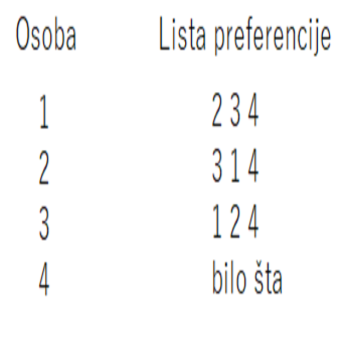
\includegraphics[width=\linewidth]{nepostoji.png}
    \caption{Nepostojeće uparivanje}
    \label{fig:nepostojece}
  \end{subfigure}
  \begin{subfigure}{0.4\textwidth}
    \centering
    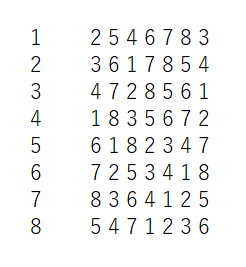
\includegraphics[width=\linewidth]{viseresenja.png}
    \caption{Postojanje više rešenja}
    \label{fig:viseresenja}
  \end{subfigure}
  \caption{Primeri instanci}
\end{figure}

\newpage

\section{Algoritam stabilnih cimera}
\label{sec:naslov1}

Algoritam se sastoji od dve faze, pri čemu obe podrazumevaju redukciju listi preferencija, dok nije zadovoljen neki kriterijum zaustavljanja. Prvi kriterijum zaustavljanja podrazumeva redukciju dok neka lista ne postane prazna, što implicira da traženo uparivanje ne postoji. Drugi kriterijum zaustavljanja je da je kardinalnost svake liste postala 1, u tom slučaju je uparivanje pronađeno, i svakoj osobi je dodeljena preostala osoba u njenoj listi. Osobe ćemo označavati brojevima od $1$ do $n$, dok će liste preferencija biti nizovi, veličine $n-1$, pri čemu za osobu $i$ lista predstavlja jednu permutaciju skupa $\{1 \ldots n\} \setminus \{i\}$.  


\subsection{Prva faza}

U prvoj fazi, krećemo se redom kroz listu osoba, i svaka od njih predlaže sledećoj osobi u svojoj listi preferencija da budu cimeri. Označimo trenutnu osobu sa $x$, a sa $y$ prvu narednu osobu iz njene liste preferencija. Ukoliko $y$ ima već predlog od neke osobe koju je rangirala više u svojoj listi preferencija, onda odbija $x$, i primorava je da nastavi sa predlozima, tamo gde je stala u svojoj listi preferencija, odnosno odmah nakon $y$. U suprotnom, $y$ nema bolji predlog od $x$, prihvata njen predlog na razmatranje, i omogućava prelazak na osobu $x+1$, koja počinje da šalje predloge osobama iz svoje liste.
\newline
Ova faza algoritma se završava ili kada svaka osoba ima predlog koji čuva, ili ukoliko je neka osoba odbijena od strane svih drugih osoba. 
\newline
Dalje u tekstu navodimo neka tvrđenja, bez dokaza, koja obezbeđuju ispravnost ove faze algoritma.

\begin{lemma}
    Ako y odbije x u nekom trenutku, onda x i y ne mogu da budu par u stabilnom uparivanju.

    \begin{corollary}
        Ako u nekom trenutku, x predloži y da budu cimeri, onda, u stabilnom uparivanju, x ne može imati boljeg partnera od y, a y ne može imati goreg od x, u kontekstu listi preferencija.
    \end{corollary}

    \begin{corollary}
        Ako je jedna osoba odbijena od strane svih, onda ne postoji stabilno uparivanje.
    \end{corollary}

    \begin{corollary}\label{posl3}
        Ako se prva faza završi tako što svaka osoba čuva predlog, onda listu preferencija osobe y, koja čuva predlog od x, možemo da redukujemo tako što brišemo sve one koji su rangirani gore od x, kao i one koji čuvaju predlog bolje rangirane osobe od y, u njihovoj listi preferencija.
    \end{corollary}
    
\end{lemma}

\begin{lemma}
    Ako u redukovanoj listi preferencija, svaka lista sadrži tačno 1 osobu, onda je to stabilno uparivanje.    
\end{lemma}

Dakle, u prvoj fazi izvodimo cikluse slanja predloga, nakon čega, na osnovu Posledice~\ref{posl3}, redukujemo liste preferencija. Ukoliko svaka lista sadrži tačno jedan element, našli smo stabilno uparivanje, u suprotnom prelazimo na drugu fazu algoritma.  

\subsection{Druga faza}
U drugoj fazi treba nekako da obradimo redukovane liste preferencija, od kojih neke liste imaju više od jednog elementa. Ponovo redukujemo liste, ali sada na nešto drugačiji način. Kriterijum zaustavljanja ostaje isti, dok nekoj osobi ne ponestane osoba kojima može da predloži da budu cimeri, ili su sve liste redukovane na tačno jednu osobu.
\newline
Ključna stvar u drugoj fazi je prepoznavanje ciklusa $a_1, a_2, ..., a_r$, različitih osoba, takvih da je druga osoba u trenutno redukovanoj listi preferencija osobe $a_i$, prva u listi preferencija osobe $a_{i+1}$, \(\forall i \in \{1, 2, \ldots, n\}\), pri čemu $i+1$ gledamo po modulu $r$. Ovakav ciklus zovemo \textit{\textbf{sve li ništa ciklus}} (\textit{eng. all or nothing cycle}).
\newline
Ispostavlja se da je lako naći jedan ovakav ciklus. Označićemo sa $p_1$ proizvoljnu osobu, čija lista preferencija ima više od jednog elementa. Koristimo niz pomoćnih promenljivih, $q_i$, pri čemu je $q_i$ druga osoba u listi preferencija od $p_i$. Na osnovu $q_i$ generišemo $p_{i+1}$, uzimajući poslednji element iz liste osobe $q_i$. Ponavljamo postupak dok niz $p$ ne napravi ciklus, odnosno dok se neka osoba ne javi dva puta. Označimo sa $p_s$ osobu koja se prva ponovila u sekvenci $p$. Niz $p_1, p_2, ..., p_s$ zovemo rep ciklusa, dok sve ili ništa ciklus dobijamo tako što $a$ uzima vrednosti na sledeći način, $a_i = p_{s+i-1}$.
\newline
Faza dva, primenjena na skup već redukovanih listi preferencija, za određeni \textit{sve ili ništa ciklus} $a_1, ..., a_r$, podrazumeva primoravanje svakog $b_i$ (prva osoba u listi od $a_i$), $1\leq i \leq r$, da odbije predlog koji čuva od $a_i$, i samim tim tera $a_i$ da pošalje predlog osobi $b_{i+1}$, drugoj osobi u njenoj trenutnoj listi preferencija. Samim tim, svi sledbenici osobe $a_i$, u redukovanoj listi preferencija osobe $b_{i+1}$ mogu biti obrisani, a takođe i $b_{i+1}$ može biti uklonjen iz njihove liste preferecija.
\newline
Značaj redukovnih listi preferencija leži u tome da, ukoliko početna instanca problema sadrži stabilno uparivanje, onda postoji i stabilno uparivanje u kojem su sve osobe uparene sa nekom iz njihove redukovane liste preferencija. Za ovakvo uparivanje kažemo da je sadržano u redukovanim listama preferencija, i ovo je posledica sledeće leme.

\begin{lemma}
        Neka je $a_1, a_2, ..., a_r$ sve ili ništa ciklus, i neka je $b_i$ prva osoba u redukovanoj listi preferencija osobe $a_i$, onda:\\

        1) U bilo kom uparivanju sadržanom u redukovanim listama preferencija, ili su $a_i$ i $b_i$ partneri za sve vrednosti $i$, ili ni za jedno.\\
        
        2) Ako postoji stabilno uparivanje u kojem su $a_i$ i $b_i$ partneri, onda postoji još jedno u kojem nisu.
        
\end{lemma}

\begin{corollary}
        Ako postoji stabilno uparivanje u početnoj instanci problema, onda postoji i stabilno uparivanje sadržano u bilo kojim redukovanim listama preferencija.
\end{corollary}

\begin{corollary}
        Ako je bilo koja od redukovanih listi preferencija prazna, onda ne postoji stabilno uparivanje.        
\end{corollary}

I poslednja i finalna lema kaže:

\begin{lemma}
    Ukoliko svaka redukovana lista preferencije sadrži tačno jednu osobu, onda postoji stabilno uparivanje za tu instancu problema.
\end{lemma}


Faza dva redukcije se sprovodi sve dok postoji lista preferencije koja ima više od jednog elementa, ili dok se neka ne isprazni, što znači da ćemo potencijalno više puta tražiti sve ili ništa cikluse i vršiti redukcije listi preferencija.

\newpage

\section{Primer primene algoritma}

U ovom poglavlju ćemo demonstrirati primenu algoritma na konkretnoj instanci problema. Liste preferencija sa kojima ćemo raditi se mogu naći u tabeli \ref{instanca}. Prva kolona označava redni broj osobe, dok se u svakoj sledećoj nalazi odgovarajuća osoba iz njene liste preferencija, pri čemu je u koloni rang 1 najbolje, a u koloni rang 5 najgore rangirana osoba.

\begin{table}[h]
    \centering
    \begin{tabular}{|c|c|c|c|c|c|}
        \hline
        Osoba & Rang 1 & Rang 2 & Rang 3 & Rang 4 & Rang 5 \\ \hline
        1 & 4 & 6 & 2 & 5 & 3 \\ \hline
        2 & 6 & 3 & 5 & 1 & 4 \\ \hline
        3 & 4 & 5 & 1 & 6 & 2 \\ \hline
        4 & 2 & 6 & 5 & 1 & 3 \\ \hline
        5 & 4 & 2 & 3 & 6 & 1 \\ \hline
        6 & 5 & 1 & 4 & 2 & 3 \\ \hline
    \end{tabular}
    \caption{Instanca problema}
    \label{instanca}
\end{table}

U prvoj fazi algoritma šaljemo predloge redom kroz liste preferencija, dok ne dođe do prihvatanja. U tom momentu smo postali favorit osobi koja nas je prihvatila, pa je važno da pamtimo favorite za svaku osobu, zbog redukcije, kao i dokle smo stigli sa slanjem predloga u listi preferencija.
\newline
\begin{itemize}
    \item Krećemo od osobe 1, ona pita osobu 4 da budu partneri.
    \begin{itemize}
        \item 4 trenutno nema favorita, pa on ne može biti bolje rangiran od 1.
        \item Sledi, 4 prihvata predlog od 1, i njen favorit postaje 1.
        \item Kraći zapis ovog koraka biće $1 - 4, f[4] = 1$, zbog kompaktnijeg zapisa kada naiđemo na suštinski isti korak.
    \end{itemize}
    \item Nastavljamo sa osobom 2, i sličnim rezonovanjem dobijamo $2 - 6, f[6] = 2$.
    \item Nakon toga, 3 pita 4 za uparivanje, ali kako je favorit osobe 4 bolje rangiran od 3, u njenoj listi preferencija, 4 odbija 3, i 3 nastavlja sa slanjem predloga kroz svoju listu. Dakle, 3 predlaže 5 uparivanje, i 5 prihvata, $f[5] = 3$.
    \item Nastavljamo dalje gde smo stali, kod osobe 4, i slično prethodnim zaključcima dobijamo $4 - 2, f[2] = 4$.
    \item Sledi, $5 - 4, f[4] = 5$, ali kako je 4 već imala favorita koji je gore rangiran od 5, ona odbija prethodnog favorita, u ovom slučaju 1, i forsira 1 da nastavi sa slanjem predloga kroz svoju listu preferencija.
    \begin{itemize}
        \item Odbijanje osobe 1 rezultuje sledećim korakom: $1 - 6, f[6] = 1$.
        \item Analogno prethodnom, 6 odbija 2, što dovodi do koraka: $2 - 3, f[3] = 2$.
    \end{itemize}
    \item Ciklus odbijanja je pokrenut iz liste osobe broj 5, pa smo njenu obradu završili, tako da nastavljamo od sledeće osobe, odnosno 6, $6 - 5, f[5] = 6$.
\end{itemize}
Kako niko nije odbijen od strane svih osoba, faza se završila tako što svako ima svog favorita, i sada možemo uraditi redukciju. Iz liste preferencija osobe $i$ možemo izbaciti sve one osobe koje su je odbile, kao i sve one koje su rangirane gore od njenog favorita, ali isto tako i svaku osobu $j$, u čijoj listi preferencija je osoba $i$ rangirana gore nego favorit osobe $j$.
\newline
\begin{itemize}
    \item Kod osobe 1 imamo da ju je odbila 4, pa nju izbacujemo. Takođe, $f[1] = 6$, pa možemo da izbacimo i 2, 5 i 3, tako da ostaje samo osoba 6 u listi.
    \item Osobu 2 je odbila 6, pa nju izbacujemo, a kako joj je favorit 4, poslednja u listi, na taj način ne možemo više ništa da eliminišemo, ali pošto je $f[1] = 6$, i bolje je rangirana od 2, možemo još da uklonimo i 1, i tako ostaju 3, 5 i 4.
    \item Dalje slično dobijamo da u listi osobe 3 ostaju 5 i 2, kod 4 ostaju 2 i 5, lista osobe 5 sadrži 4, 2 i 3, dok kod 6 ostaje samo 1.
\end{itemize}
Redukovane liste preferencija nakon prve faze možemo videti u tabeli \ref{redukovane}.
Pošto još uvek postoje liste preferencija koje imaju više od jednog elementa, prelazimo na drugu fazu. Za to nam je potrebno da generišemo \textit{sve ili ništa ciklus}.
Uzećemo recimo da je početna osoba 2, tj $p_1 = 2$. Na osnovu već opisane procedure, $q_1$ dobijamo kao drugu osobu iz liste $p_1$, tako da je $q_1 = 5$. Sada nam treba $p_2$, nju nalazimo kao poslednju osobu u listi od $q_1$, dakle $p_2 = 3$. Analogno ovome dobijamo, $q_2 = 2, p_3 = 4, q_3 = 5, p_4 = 3$. U ovom trenutku osoba 3 se javila dva puta, pa je sekvenca formirala ciklus, i naš traženi ciklus je 3, 4. Kao što je opisano ranije u tekstu, svaka osoba iz ciklusa biva odbijena od prve osobe u svojoj redukovanoj listi preferencija, i time je primorana da šalje predlog sledećoj osobi. Samim tim, 3 je odbijena od strane 5, i šalje predlog osobi broj 2, pa 5 može biti uklonjena iz liste, pa ostaje samo 2. Dalje, pošto je sada favorit od 2 osoba broj 3, sve nakon nje mogu biti uklonjene, pa tako brišemo 5 i 4, i u listi osobe 2 ostaje samo 3.
\newline
Isto ovo primenjujemo i za osobu 4, koja je sledeća u ciklusu, i kao rezultat iz njene liste uklanjamo 2, te ostaje samo 5, a iz liste osobe 5 uklanjamo sve nakon 4, tj. 2 i 3, pa ostaje samo 4. Ovim su sve liste preferencija svedene na 1 element, što znači da je uparivanje pronađeno, i svakoj osobi je dodeljena jedina preostala u njenoj listi. Traženo uparivanje je $1 - 6, 2 - 3, 4 - 5$.
\newline
U opštem slučaju, redukcija faze 2 će možda morati da se primeni više puta, ali je u ovom primeru kriterijum zaustavljanja zadovoljen nakon jedne primene.

\begin{table}[h]
    \centering
    \begin{tabular}{|c|c|c|c|c|c|}
        \hline
        Osoba & Rang 1 & Rang 2 & Rang 3\\ \hline
        1 & 6 &  &  \\ \hline
        2 & 3 & 5 & 4 \\ \hline
        3 & 5 & 2 & \\ \hline
        4 & 2 & 5 & \\ \hline
        5 & 4 & 2 & 3 \\ \hline
        6 & 1 &  & \\ \hline
    \end{tabular}
    \caption{Redukovane liste preferencija}
    \label{redukovane}
\end{table}

\newpage
\section{Implementacija}
Algoritam je implementiran u programskom jeziku C++, a kako bi korišćenje bilo olakšano, integrisan je u aplikaciju napravljenu pomoću alata QtCreator. U ovom poglavlju biće opisane samo najbitnije funkcije i strukture podataka za rad algoritma, dok će opisivanje integracije algoritma u Qt aplikaciju biti zanemareno.


Za opisivanje matrice preferencija, koju zovemo \textit{preferences} koristimo \\ ugrađenu strukturu podataka jezika C++, vector, tačnije vektor vektora. Na samom početku, tokom unosa instance problema, odnosno matrice preferencija, formiramo i matricu \textit{rankings}, koja predstavlja rangove osoba u listama preferencija. Preciznije, $rankings[i][j]$ predstavlja poziciju osobe $j$ u listi preferencija osobe $i$. Ovo nam olakšava posao, jer će nam rangovi biti potrebni, kod prihvatanja ili odbijanja predloga za uparivanje, a njihovo računanje tokom algoritma bi oduzimalo bespotrebno vreme.


U nastavku slede opisi najvažnijih funkcija, nakon kojih se mogu naći i pseudokodovi.
\newline
\textbf{do\_proposals} - Ovo je pomoćna funkcija koja služi za realizaciju prve faze algoritma, kako bi kod bio čitljiviji. Argumenti funkcije su \textit{preferences, rankings, favorites, proposals\_pos, roommate, n}. Vektor \textit{favorites} pamti za svaku osobu njenog trenutnog favorita, odnosno najbolje rangiranu osobu u njenoj listi preferencija, od koje je dobila predlog za uparivanje. Vektor \textit{proposals\_pos} čuva poziciju u listi preferencija do koje se stiglo sa slanjem predloga, za svaku osobu. Ceo broj \textit{roommate} označava osobu za koju se vrši slanje predloga do prihvatanja, a $n$ dimenziju problema. Funkcija ide redom kroz listu preferencija osobe \textit{roommate}, i šalje predloge za uparivanje, sve dok neko ne prihvati, a to bi značilo da \textit{roommate} ima bolji rang u listi preferencija osobe koja prihvata predlog, od njenog trenutnog favorita. Samim tim, favorit se ažurira, a za bivšeg favorita se rekurzivno poziva funkcija. Ukoliko se stiglo do kraja liste preferencija neke osobe, znači da je ona odbijena od strane svih ostalih, i algoritam nema stabilno uparivanje, pa se prekida izvršavanje.

\begin{figure}[H]
    \centering
    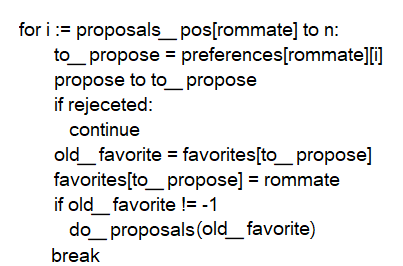
\includegraphics[width=0.4\textwidth]{do_proposals.png}
    \caption{Funkcija do\_proposals}
    \label{doprop}
\end{figure}

\textbf{stage\_one} - Funkcija realizuje prvu fazu redukcija listi preferencija, pozivajući funkciju \textit{do\_proposals} za svaku osobu, kako bi odredila favorite. Nakon toga, na osnovu favorita vrši redukciju listi preferencija na način opisan ranije u tekstu. Argumenti funkcije su isti kao za prethodnu, osim što ne prima određenu osobu.

\begin{figure}[H]
    \centering
    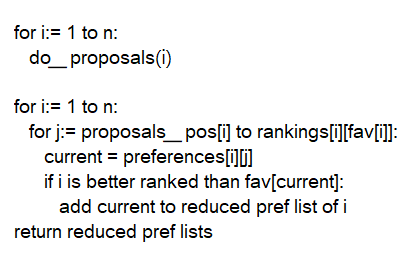
\includegraphics[width=0.4\textwidth]{stage one.png}
    \caption{Funkcija stage\_one}
    \label{so}
\end{figure}

\textbf{phase\_two\_condition} - Funkcija prostim prolaskom kroz liste preferencija proverava da li je neki od ranije opisanih uslova za zaustavljanje druge faze algoritma zadovoljen.


\begin{figure}[H]
    \centering
    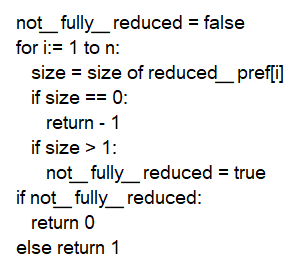
\includegraphics[width=0.3\textwidth]{p2condition.png}
    \caption{Funkcija phase\_two\_condition}
    \label{p2c}
\end{figure}

\textbf{find\_all\_or\_nothing\_cycle} - Nalazi traženi ciklus, prema opisanoj proceduri, tako što početni element bira na slučajan način, i smešta ga u vektor \textit{cycle}, a vraća veličinu repa kao povratnu vrednost. Ukoliko funkcija mora biti pozvana više puta, odnosno izvršava se više redukcija druge faze, onda se za početnu osobu bira poslednja osoba iz repa prethodnog ciklusa. Ovo je zbog toga što njene liste preferencija nisu obuhvaćene redukcijom druge faze, pa i dalje ima više od jedne osobe u listi, što ubrzava traženje odgovarajuće osobe za generisanje ciklusa.

\begin{figure}[H]
    \centering
    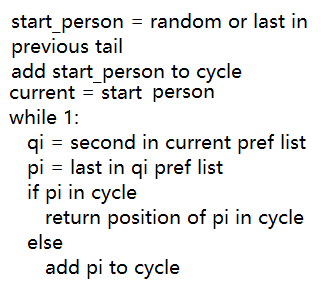
\includegraphics[width=0.3\textwidth]{allornothingcycle.png}
    \caption{Funkcija find\_all\_or\_nothing\_cycle}
    \label{allorn}
\end{figure}

\textbf{phase\_two\_reduction} - Vrši redukciju druge faze na osnovu jednog ciklusa, krećući se po generisanom ciklusu, i uklanjajući odgovarajuće osobe iz listi preferencija, na već ranije opisan način.

\begin{figure}[H]
    \centering
    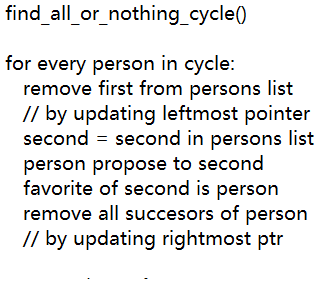
\includegraphics[width=0.35\textwidth]{p2reduction.png}
    \caption{Funkcija phase\_two\_reduction}
    \label{p2r}
\end{figure}

\textbf{stable\_roommates\_algorithm} - Kombinuje obe faze u jednu celinu, vršeći redukciju prve faze, i potom dok god nije ispunjen uslov za zaustavljanje druge faze, poziva funkciju \textit{phase\_two\_reduction}, izvršavajući jednu redukciju druge faze.

\begin{figure}[H]
    \centering
    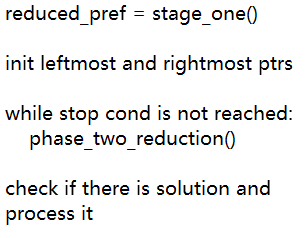
\includegraphics[width=0.3\textwidth]{stableroommates.png}
    \caption{Funkcija stable\_roommates\_algorithm}
    \label{sra}
\end{figure}

\section{Složenost}
Analiziraćemo posebno složenost prve i druge faze.
\subsection{Prva faza}
Prva faza se sastoji od poziva funkcije \textbf{do\_proposals}. Kako ona uvek nastavlja izvršavanje od mesta na kom je zaustavljeno slanje predloga u nekom prošlom pozivu, i nikad se ne vraća unazad kroz liste preferencija, najgori slučaj je da je neko odbijen od strane svih ostalih, a ostali su stigli da pretposlednje osobe u svojim listama preferencija. Stoga je maksimalan broj koraka reda veličine matrice, a kako su ostale operacije složenosti $O(1)$, složenost ove faze algoritma reda $O(n^2)$.
\subsection{Druga faza}
Druga faza se sastoji od generisanja \textit{sve ili ništa ciklusa}, i redukcije liste preferencija na ranije opisani način, dok neki kriterijum zaustavljanja ne bude zadovoljen. Proveru uslova vršimo uz pomoć tehnike dva pokazivača, održavajući dva vektora, \textit{leftmost} i \textit{rightmost}, koji pokazuju na najlevlji i najdešnji element u listi preferencija svake osobe. Ovako je provera veličine liste preferencija neke osobe, odnosno zadovoljenja nekog uslova zaustavljanja, složenosti $O(1)$. Nakon svake redukcije druge faze ažuriramo na odgovarajući način ova dva vektora. Kako je, hipotetički, maksimalan broj elemenata koji mogu biti izbačeni tokom druge faze $n^2$, a složenost ostalih operacija, i generisanja ciklusa $O(1)$, sledi da je maksimalan broj koraka reda $O(n^2)$, samim tim je i složenost celog algoritma $O(n^2)$.

\section{Rezultati}
U ovom delu biće ukratko predstavljeni rezultati rada algoritma, dobijeni testiranjem algoritma na slučajno odabranim instancama problema. Sva testiranja sprovedena su na 1000 različitih instanci, za različite dimenzije ulaza. Dobijeni rezultati su predstavljeni u Tabeli \ref{tab:problemi}, gde možemo videti broj instanci sa rešenjem kao i prosečno vreme izvršavanja u mikrosekundama, za testirane instance.

\begin{table}[H]
  \centering
  \begin{tabular}{cccc}
    \toprule
    Dimenzija & Broj instanci & Broj sa rešenjem & Vreme (ms)\\
    \midrule
    4 & 1000 & 966 & 5 \\
    6 & 1000 & 924 & 3 \\
    8 & 1000 & 879 & 5 \\
    10 & 1000 & 823 & 7 \\
    12 & 1000 & 776 & 12 \\
    14 & 1000 & 706 & 16 \\
    16 & 1000 & 626 & 20 \\
    18 & 1000 & 583 & 19 \\
    20 & 1000 & 500 & 17 \\
    22 & 1000 & 441 & 36 \\
    24 & 1000 & 408 & 32 \\
    \bottomrule
  \end{tabular}
  \caption{Rezultati rada algoritma}
  \label{tab:problemi}
\end{table}

\section{Zaključak}
\label{sec:zakljucak}

U ovom tekstu smo razmotrili problem \textit{stabilnih cimera}, kao i algoritam za njegovo rešavanje. Nakon predstavljanja implementacije u C++u, analizirali smo složenost i zaključili da je u najgorem slučaju ona reda $O(n^2)$, što je efikasan i praktično upotrebljiv algoritam. Veći problem od samog vremena prave memorijski zahtevi za veliko $n$, pošto treba skladištiti veći broj dodatnih struktura podataka.\\
Kako postoji efikasan algoritam, ovaj problem bi mogao da nađe i praktične primene, kao na primer kod raspoređivanja studenata u domovima, ili kod raznih društvenih mreža i aplikacija za upoznavanje, gde bi ljudi bili povezivani prema njihovim interesima, hobijima i preferencijama.




\addcontentsline{toc}{section}{Literatura}
\appendix
\bibliography{seminarski} 
\bibliographystyle{plain}


\end{document}
